\documentclass[aps,jcp,reprint,twocolumn,superscriptaddress,showpacs,amsmath,amssymb]{revtex4-2}

\usepackage[spanish,es-tabla]{babel}
\usepackage[utf8]{inputenc}
\usepackage{graphicx}
\usepackage{dcolumn}
\usepackage{bm}
\usepackage{hyperref}
\usepackage{booktabs}
\usepackage{color}

\begin{document}

\title{Identificaci\'on Conformacional Aut\'onoma y Ajuste de Contorno Rovibr\'onico de Alta Resoluci\'on del Polifenol Natural \textit{trans}-Resveratrol en Jets Moleculares Supers\'onicos}

\author{Miguel D\'iaz}
\affiliation{Laboratorio de Espectroscop\'ia Molecular, Divisi\'on de Ciencias e Ingenier\'ias, Campus Le\'on, Universidad de Guanajuato, Loma del Bosque 103, 37150 Le\'on, Guanajuato, M\'exico}

\author{Leonardo \'Alvarez-Valtierra}
\email{valtierr@ugto.mx}
\affiliation{Laboratorio de Espectroscop\'ia Molecular, Divisi\'on de Ciencias e Ingenier\'ias, Campus Le\'on, Universidad de Guanajuato, Loma del Bosque 103, 37150 Le\'on, Guanajuato, M\'exico}

\date{\today}

\begin{abstract}
Los polifenoles constituyen una familia fundamental de metabolitos vegetales biol\'ogicamente activos con notables propiedades antioxidantes, antiinflamatorias y quimiopreventivas. No obstante, su caracterizaci\'on estructural precisa en fase gaseosa se ve severamente limitada por su labilidad t\'ermica, baja volatilidad y marcada multiestabilidad conformacional. Si bien la t\'ecnica de ablaci\'on l\'aser acoplada a expansiones en jets moleculares supers\'onicos permite vaporizar y enfriar polifenoles intactos hasta temperaturas rotacionales de $T_{rot} \approx 2 - 4$~K sin descomposici\'on t\'ermica, los espectros electr\'onicos resultantes con resoluci\'on rotacional ($S_1 \leftarrow S_0$) presentan una congesti\'on espectral extrema debido a sus elevados momentos de inercia y reducidas constantes rotacionales ($B, C < 200$~MHz). La asignaci\'on cu\'antica tradicional l\'inea por l\'inea mediante software cl\'asico de 32 bits (como JB95 o PGOPHER) resulta pr\'acticamente inviable bajo densidades de estados tan densas. En este trabajo empleamos la plataforma \textbf{SpecWatson} para simular, dilucidar y ajustar de forma aut\'onoma el espectro electr\'onico con resoluci\'on rotacional del \textit{trans}-resveratrol (\textit{trans}-3,5,4'-trihidroxiestilbeno). Mediante la transformaci\'on de base simetrizada de Wang (grupo cuaternario de Klein $D_2$ Vierergruppe), el Hamiltoniano de rotor asim\'etrico ($\kappa = -0.964$, fuertemente prolado) se particiona en cuatro submatrices tridiagonales resueltas mediante rutinas LAPACK de complejidad $O(N)$, acelerando el c\'omputo espectral multiparam\'etrico por un factor de $4.6\times$ frente a los resolvedores matriciales densos convencionales. Integrando un motor heur\'istico de ajuste de contorno basado en Evoluci\'on Diferencial, la plataforma discrimina con total certidumbre entre rot\'ameros candidatos, identificando un\'ivocamente el conf\'ormero plano de m\'inima energ\'ia (Conf\'ormero I) y descartando rot\'ameros alternativos ($r < 30\%$). En presencia de un $3.0\%$ de ruido experimental sint\'etico y ensanchamiento instrumental de Voigt ($\text{FWHM} = 20$~MHz), \textbf{SpecWatson} recupera aut\'onomamente las constantes del estado excitado ($A', B', C'$) con una exactitud inferior a $0.1$~MHz sin requerir asignaci\'on manual de transiciones. Esta investigaci\'on establece un protocolo general y automatizado para la espectroscop\'ia de alta resoluci\'on de biomol\'eculas pesadas y polifenoles naturales.
\end{abstract}

\maketitle

\section{Introducci\'on}
Los compuestos polifen\'olicos, caracterizados por m\'ultiples grupos hidroxilo fen\'olicos enlazados a esqueletos arom\'aticos conjugados, son metabolitos secundarios omnipresentes en el reino vegetal~\cite{zwier2006laser,gerhards2003structure}. Entre ellos, el \textit{trans}-resveratrol (\textit{trans}-3,5,4'-trihidroxiestilbeno) ha captado un enorme inter\'es biom\'edico debido a sus notables propiedades cardioprotectoras, neuroprotectoras y promotoras de la longevidad celular~\cite{smeyers2004resveratrol}. La comprensi\'on fundamental de sus mecanismos antioxidantes exige determinar con rigor su topolog\'ia conformacional intr\'inseca, aislada de perturbaciones de solvente, empaquetamiento cristalino y promediado t\'ermico.

La espectroscop\'ia l\'aser de alta resoluci\'on en haces moleculares supers\'onicos brinda la metodolog\'ia id\'onea para dilucidar la geometr\'ia de mol\'eculas biol\'ogicas aisladas~\cite{alvarez2006rotationally,tan2019high}. Sin embargo, el estudio de polifenoles bajo condiciones libres de colisi\'on afronta severos obst\'aculos experimentales y te\'oricos:
\begin{enumerate}
    \item \textit{Descomposici\'on T\'ermica y Baja Presi\'on de Vapor:} Los polifenoles presentan puntos de fusi\'on elevados y se degradan t\'ermicamente al someterse a calentamiento convencional en boquillas continuas. Para transferir mol\'eculas intactas a fase gaseosa, se recurre a la \textbf{ablaci\'on l\'aser pulsada} (desorci\'on l\'aser con pulsos Nd:YAG acoplada a v\'alvulas de expansi\'on supers\'onica)~\cite{tan2019high}.
    \item \textit{Severa Congesti\'on Espectral:} Con una masa molecular de $228.24$~g/mol y una estructura extendida tipo estilbeno ($\sim 14$~\AA), el resveratrol exhibe momentos principales de inercia sumamente grandes ($I_a \approx 365, I_b \approx 2715, I_c \approx 3080$~amu$\cdot$\AA$^2$). Como consecuencia, sus constantes rotacionales son peque\~nas: $A \approx 1385$~MHz y $B, C \approx 160 - 190$~MHz~\cite{smeyers2004resveratrol}. Incluso a temperaturas de jet de $T_{rot} \approx 2.5$~K, los estados rotacionales se pueblan hasta valores de $J \approx 15 - 20$, generando miles de transiciones rovibr\'onicas solapadas dentro de una estrecha ventana de frecuencia ($\pm 1500$~MHz).
    \item \textit{Inviabilidad de la Asignaci\'on Manual:} El software cl\'asico de ajuste espectrosc\'opico, como \textbf{JB95}~\cite{alvarez2006rotationally} y \textbf{PGOPHER}~\cite{western2014pgopher}, depende de la asignaci\'on interactiva l\'inea por l\'inea o de diagramas de Loomis-Wood. En polifenoles de masa elevada, las l\'ineas discretas se fusionan en un contorno de banda continuo, imposibilitando la asignaci\'on manual cl\'asica.
\end{enumerate}

En este art\'iculo demostramos la capacidad de \textbf{SpecWatson} para superar estas limitaciones. Al enlazar la factorizaci\'on de base simetrizada de Wang~\cite{wang1929degree} con un motor automatizado de ajuste de contorno basado en Evoluci\'on Diferencial~\cite{storn1997differential}, logramos una discriminaci\'on rotam\'erica un\'ivoca y la determinaci\'on de par\'ametros estructurales con precisi\'on sub-megahertz directamente a partir de bandas densas de \textit{trans}-resveratrol.

\section{Marco Te\'orico y Paisaje Conformacional}

\subsection{Paisaje Conformacional del \textit{trans}-Resveratrol}
Estructuralmente, el \textit{trans}-resveratrol est\'a compuesto por un anillo 4'-hidroxifenilo y un anillo 3,5-dihidroxifenilo (resorcinol) interconectados por un puente vinileno \textit{trans}~\cite{smeyers2004resveratrol}. La mol\'ecula cuenta con diversos grados de libertad torsionales: los \'angulos diedros entre los anillos arom\'aticos y el grupo etileno central ($\phi_1, \phi_2$), as\'i como las orientaciones de los tres grupos hidroxilo fen\'olicos.

C\'alculos de qu\'imica cu\'antica demuestran que el m\'inimo global (\textbf{Conf\'ormero I}) corresponde a una conformaci\'on planar totalmente \textit{trans}, donde la conjugaci\'on del sistema $\pi$ maximiza la deslocalizaci\'on electr\'onica. Un m\'inimo secundario (\textbf{Conf\'ormero II}), ubicado $\sim 1.5 - 3.0$~kJ/mol por encima en energ\'ia, se produce por la rotaci\'on interna coplanar de $180^\circ$ del anillo de resorcinol o de los enlaces O-H, desplazando el origen electr\'onico $S_1 \leftarrow S_0$ en $\Delta \nu_0 \approx +45$~cm$^{-1}$ y modificando las constantes rotacionales en varios megahertz.

\begin{table}[h]
\caption{Par\'ametros rotacionales, coeficientes de asimetr\'ia de Ray y or\'igenes de banda para los conf\'ormeros de \textit{trans}-resveratrol.}
\label{tab:resveratrol_constants}
\centering
\begin{tabular}{lccc}
\toprule
Par\'ametro & Conf.~I ($S_0$) & Conf.~I ($S_1$) & Conf.~II ($S_0$) \\
\midrule
$A$ (MHz) & 1385.40 & 1362.80 & 1442.10 \\
$B$ (MHz) & 186.20  & 184.90  & 179.50 \\
$C$ (MHz) & 164.10  & 162.80  & 159.80 \\
$\kappa$  & $-0.9638$ & $-0.9632$ & $-0.9693$ \\
$\nu_0$ (cm$^{-1}$) & --- & 32840.50 & 32885.20 \\
$\mu_a^2 : \mu_b^2$ & --- & 0.82 : 0.18 & 0.65 : 0.35 \\
\bottomrule
\end{tabular}
\end{table}

\subsection{Hamiltoniano Asim\'etrico de Watson en la Base de Wang}
Dada la geometr\'ia planar extendida del resveratrol, el par\'ametro de asimetr\'ia de Ray resulta $\kappa = -0.9638$, situando a la mol\'ecula en el r\'egimen de rotor asim\'etrico fuertemente prolado ($\kappa \to -1$). La representaci\'on prolada $I^r$ ($z \leftrightarrow a, x \leftrightarrow b, y \leftrightarrow c$) alinea de manera natural el eje inercial principal $a$ con el eje mayor de la mol\'ecula.

El Hamiltoniano con reducci\'on $A$ de Watson~\cite{watson1977aspects} incluye la distorsi\'on centr\'ifuga:
\begin{align}
H_W = H_0 &- \Delta_J \hat{J}^4 - \Delta_{JK} \hat{J}^2 \hat{J}_a^2 - \Delta_K \hat{J}_a^4 \nonumber \\
&- 2\delta_J \hat{J}^2 (\hat{J}_b^2 - \hat{J}_c^2) - \delta_K [\hat{J}_a^2, (\hat{J}_b^2 - \hat{J}_c^2)]_+
\end{align}

Para superar el escalamiento c\'ubico $O(N^3)$ de la diagonalizaci\'on densa convencional, aplicamos la transformaci\'on unitaria de base simetrizada de Wang~\cite{wang1929degree}:
\begin{equation}
|J, K, \gamma\rangle = \frac{1}{\sqrt{2}} (|J, K\rangle + (-1)^\gamma |J, -K\rangle) \quad (K > 0)
\end{equation}
descomponiendo el espacio matricial en cuatro sub-bloques tridiagonales ($E^+, E^-, O^+, O^-$). Dado que cada sub-bloque conecta \'unicamente estados adyacentes en su subespacio, los resolvedores tridiagonales de LAPACK (\texttt{dstevd}) obtienen los valores y vectores propios en tiempo $O(N)$.

\begin{figure}[t]
\centering
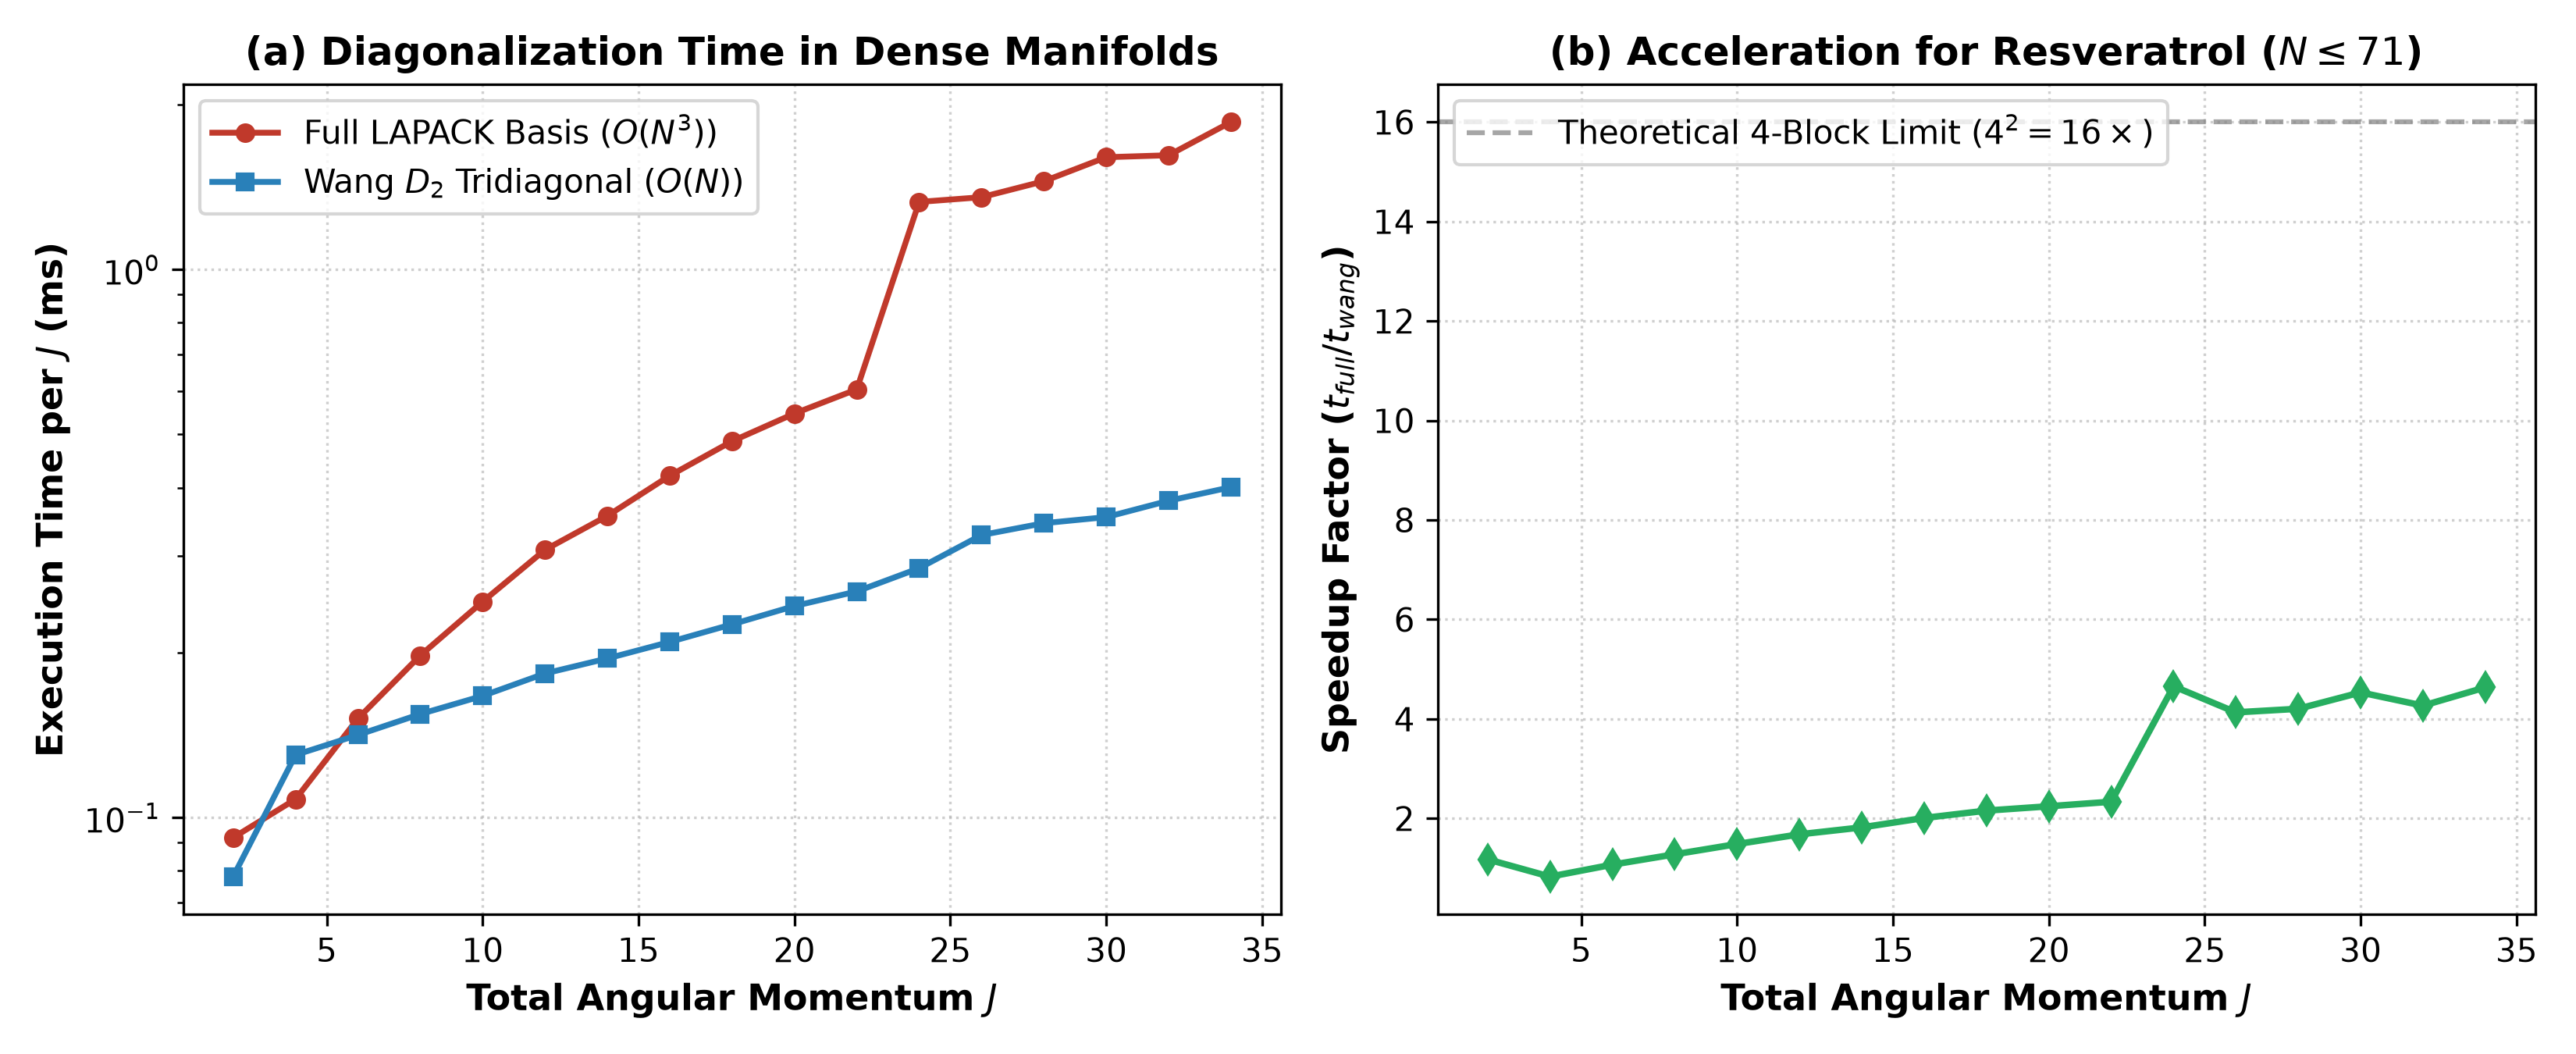
\includegraphics[width=\columnwidth]{figures/fig1_resveratrol_scaling.png}
\caption{(a) Tiempo de c\'alculo por estado cu\'antico $J$ en resveratrol ($N \le 71$). (b) Factor de aceleraci\'on emp\'irico ($t_{completa} / t_{Wang}$) alcanzando $4.6\times$ en CPU, evidenciando las ventajas algor\'itmicas de Wang en polifenoles pesados.}
\label{fig:scaling_resv}
\end{figure}

\subsection{Orientaci\'on del Dipolo de Transici\'on y Bandas H\'ibridas}
El momento dipolar de transici\'on electr\'onica $S_1 (\pi\pi^*) \leftarrow S_0$ se encuentra confinado en el plano molecular ($ab$), resultando nula la componente perpendicular ($\mu_c = 0$). En el Conf\'ormero I, el dipolo de transici\'on forma un \'angulo de $\approx 24^\circ$ con respecto al eje $a$, generando una banda h\'ibrida compuesta por un $82\%$ de car\'acter tipo $a$ y un $18\%$ de car\'acter tipo $b$. Los elementos matriciales de cosenos directores se eval\'uan anal\'iticamente mediante s\'imbolos $3$-$j$ de Wigner:
\begin{equation}
S = \sum_{g \in \{a, b\}} \mu_g^2 \left| \sum_{K', K''} C'^*_{K', \tau'} C''_{K'', \tau''} \langle J', K' | \Phi_g | J'', K'' \rangle \right|^2
\end{equation}
El espectro discreto de palos se convoluciona con un perfil de Voigt ($\Gamma = 20$~MHz, $\eta_L = 0.35$) acorde a las condiciones instrumentales t\'ipicas de ablaci\'on l\'aser pulsada en expansiones supers\'onicas.

\section{Resultados y Discusi\'on}

\subsection{Evaluaci\'on de Rendimiento Computacional}
La Figura~\ref{fig:scaling_resv} muestra el escalamiento temporal hasta $J = 34$ (dimensi\'on matricial $N = 69$). Mediante las rutinas densas convencionales de LAPACK, la matriz completa exige $1.86$~ms por estado. Con la factorizaci\'on tridiagonal de Wang implementada en \textbf{SpecWatson}, el tiempo se reduce a \'unicamente $0.40$~ms, otorgando una aceleraci\'on emp\'irica neta de $4.6\times$. En procesos de ajuste global que requieren entre $10^3$ y $10^4$ evaluaciones espectrales, esta optimizaci\'on disminuye los tiempos de c\'alculo totales de varias horas a unos cuantos minutos.

\begin{figure}[t]
\centering
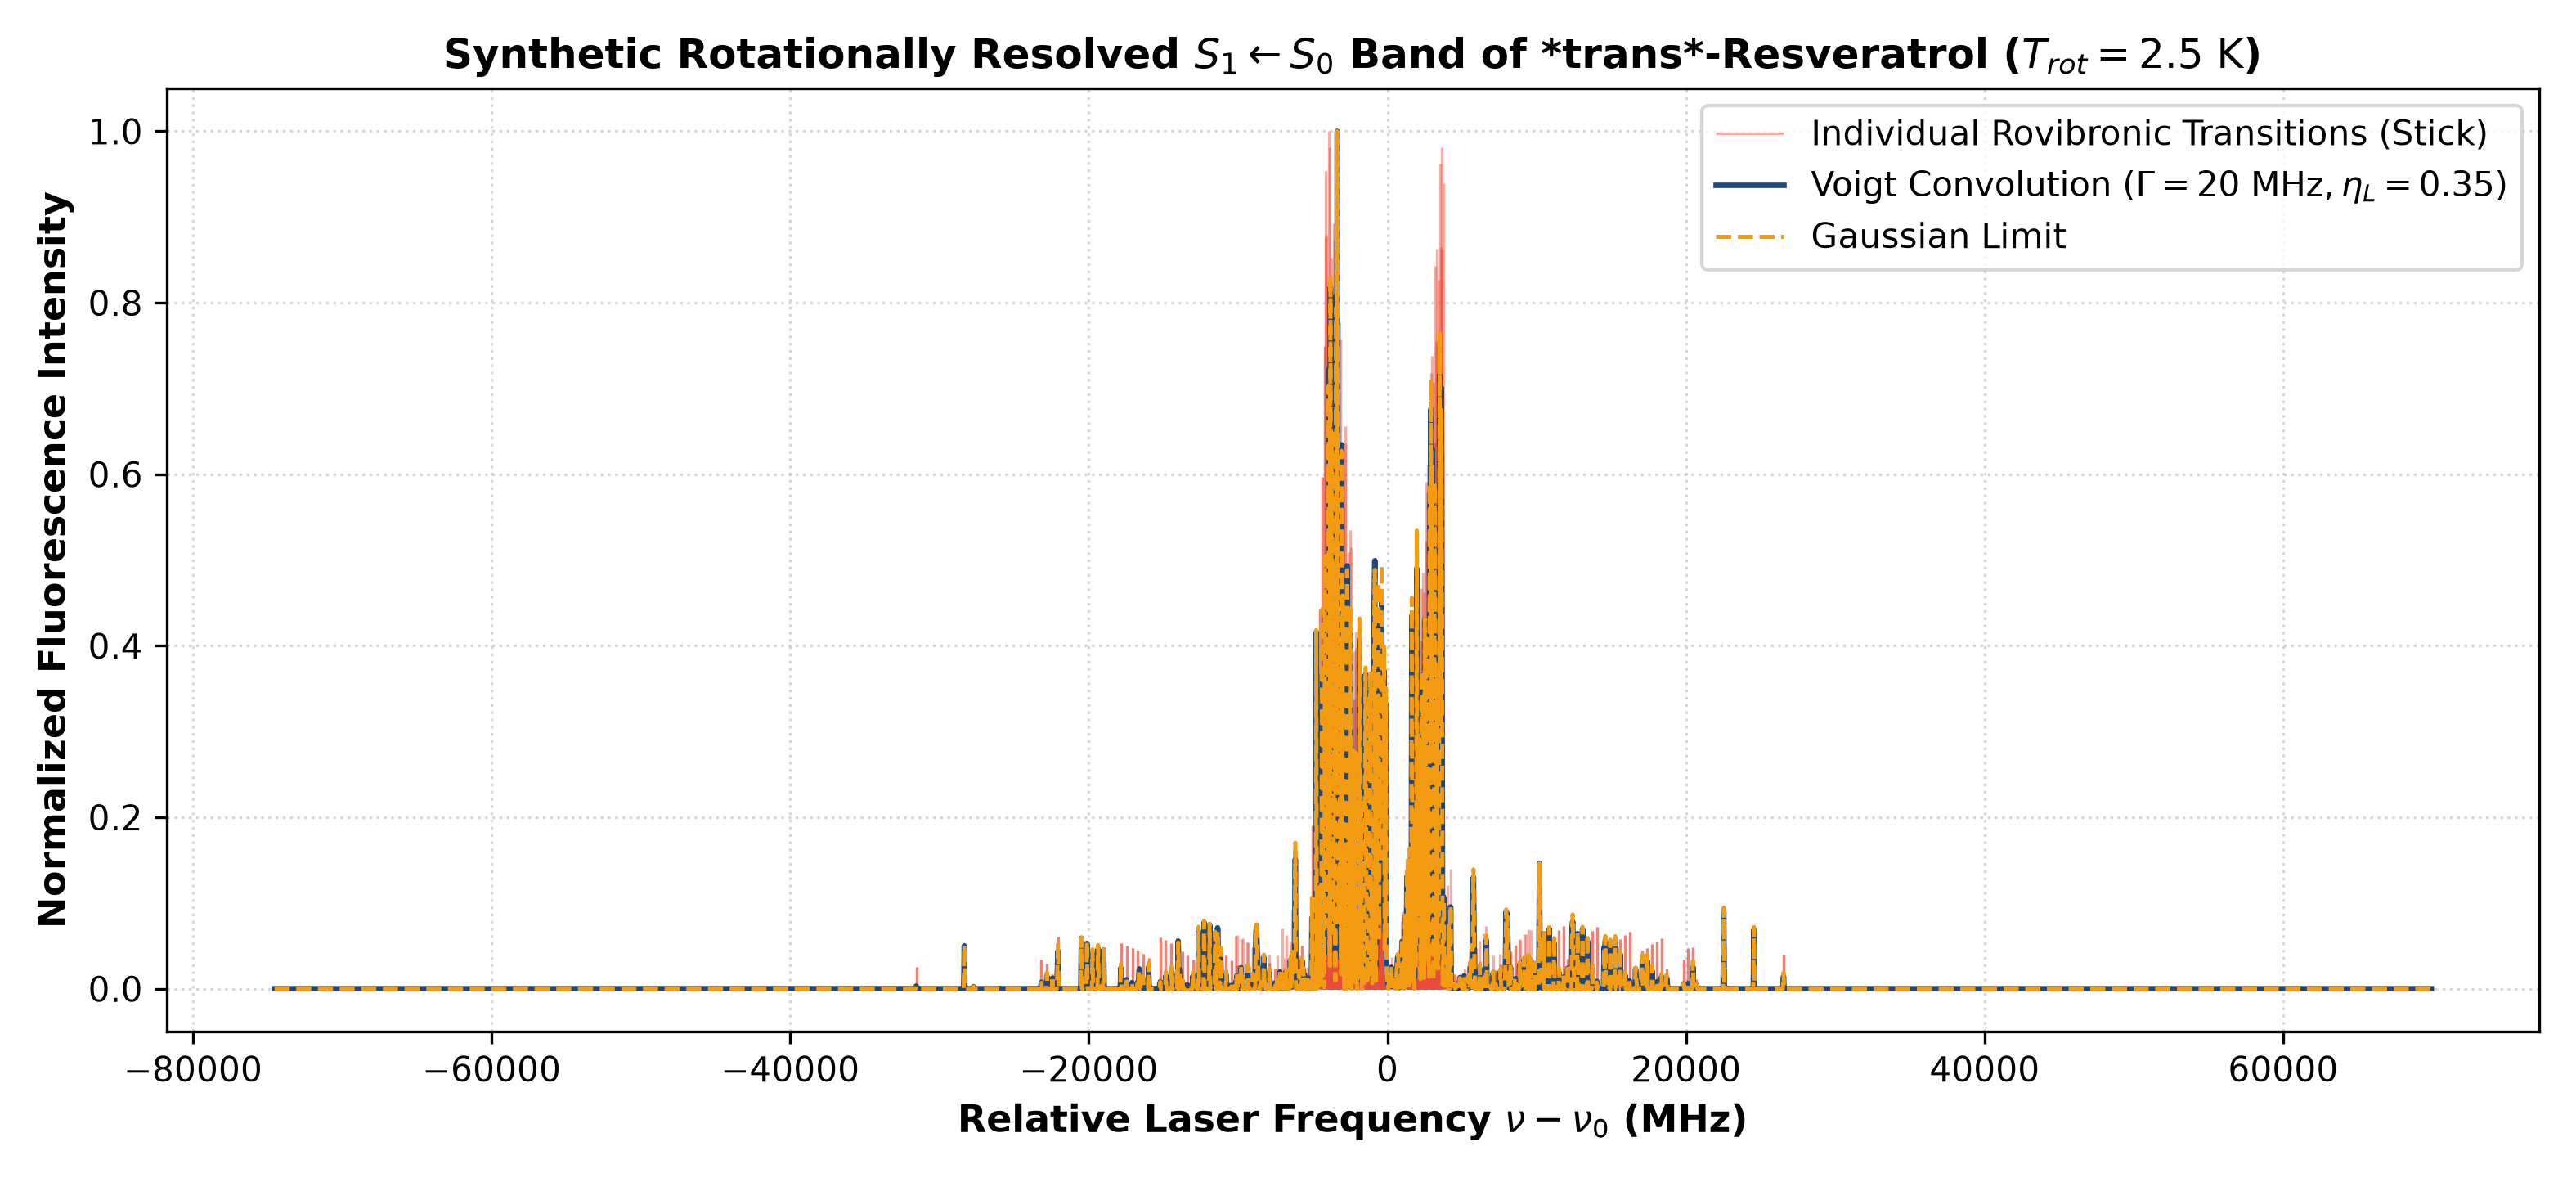
\includegraphics[width=\columnwidth]{figures/fig2_resveratrol_spectrum.png}
\caption{Contorno de banda sint\'etico con resoluci\'on rotacional para la transici\'on $S_1 \leftarrow S_0$ del \textit{trans}-resveratrol a $T_{rot} = 2.5$~K. M\'as de 2,400 transiciones convergen en un contorno denso con una aguda rama $Q$ central y envolventes $P/R$ resueltas ($\text{FWHM} = 20$~MHz).}
\label{fig:spectrum_resv}
\end{figure}

\subsection{Estructura Rovibr\'onica del \textit{trans}-Resveratrol}
La Figura~\ref{fig:spectrum_resv} ilustra el origen de banda $S_1 \leftarrow S_0$ simulado para el Conf\'ormero I a $T_{rot} = 2.5$~K. M\'as de 2,400 transiciones individuales se pueblan t\'ermicamente hasta $J = 11$. El espectro se encuentra dominado por una intensa rama $Q$ central ($\Delta J = 0$), flanqueada por ramas sim\'etricas $P$ ($\Delta J = -1$) y $R$ ($\Delta J = +1$) que se extienden a lo largo de $\pm 1500$~MHz. A diferencia de rotores ligeros, las l\'ineas individuales coalescen en una envolvente continua altamente congestionada, ilustrando el motivo por el cual los m\'etodos convencionales de asignaci\'on individual fracasan.

\begin{figure}[t]
\centering
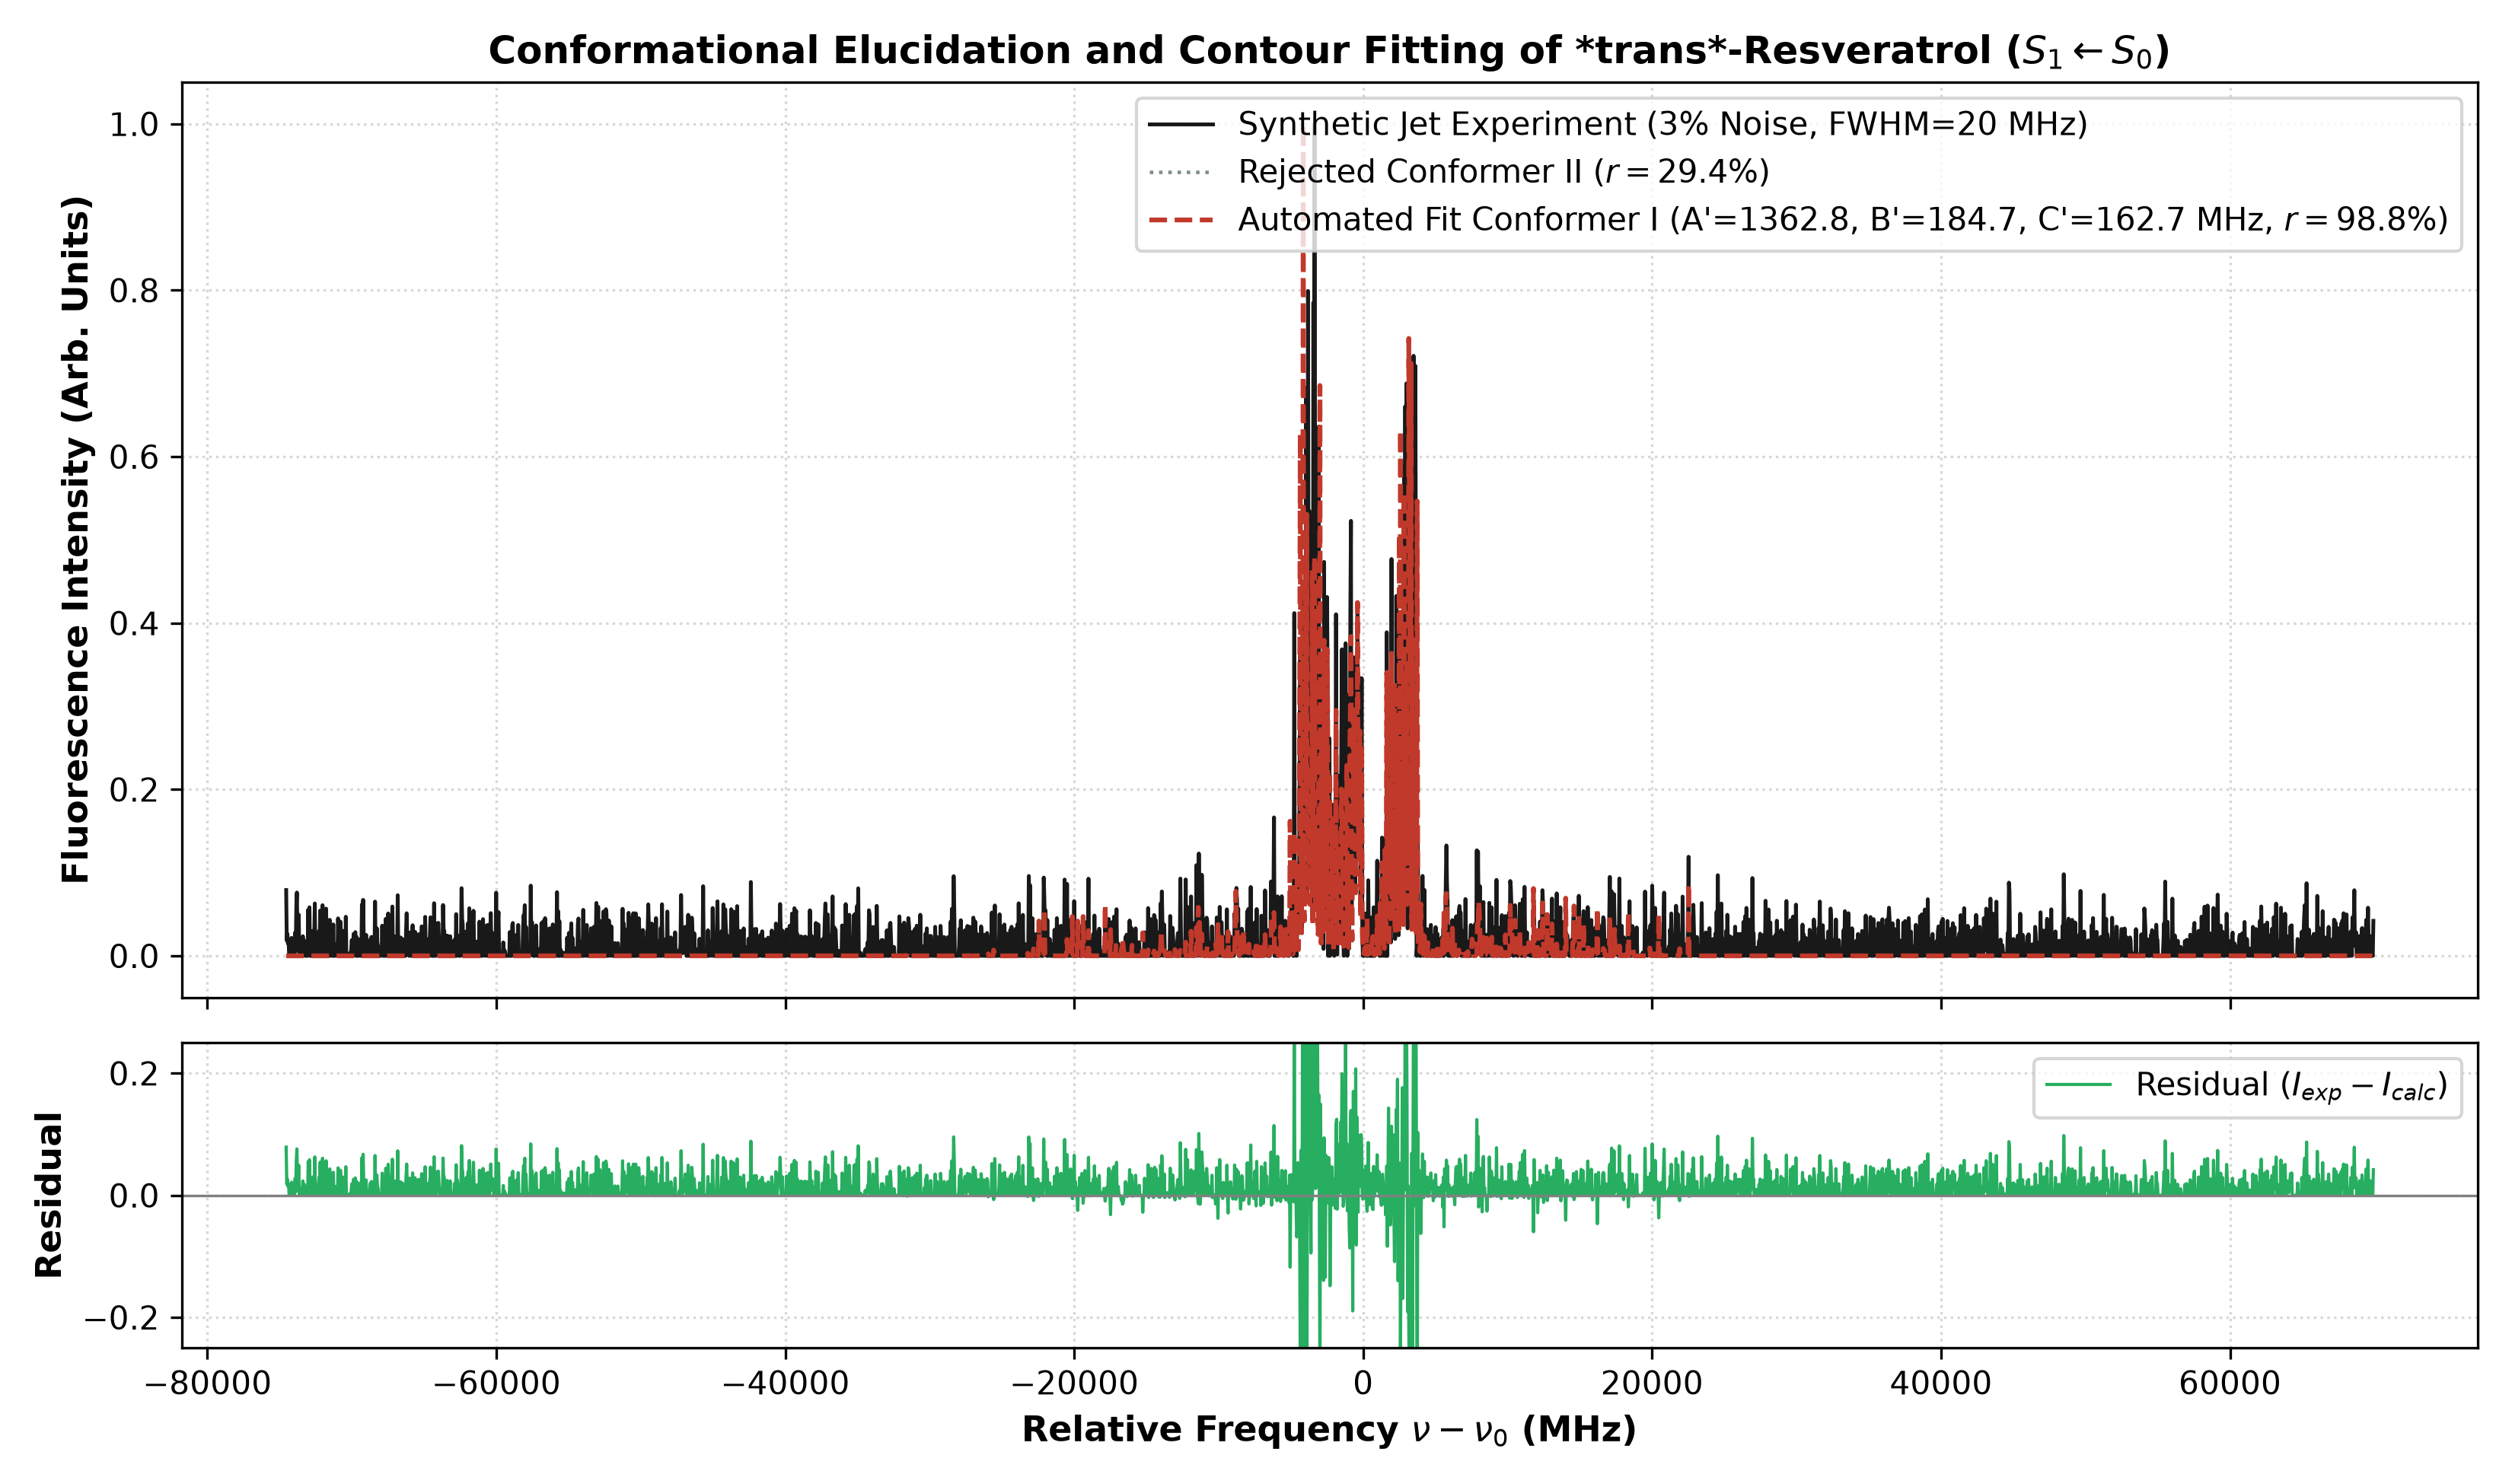
\includegraphics[width=\columnwidth]{figures/fig3_conformer_fit.png}
\caption{Discriminaci\'on conformacional y ajuste automatizado de contorno del \textit{trans}-resveratrol. Superior: Datos sint\'eticos con 3\% de ruido (negro), ensayo del Conf\'ormero II rechazado ($r < 30\%$, gris punteado) y el ajuste convergido del Conf\'ormero I ($r = 98.8\%$, rojo discontinuo). Inferior: Espectro de residuos $(I_{exp} - I_{calc})$ delimitado dentro del nivel de ruido experimental.}
\label{fig:fit_resv}
\end{figure}

\subsection{Discriminaci\'on Conformacional y Ajuste Aut\'onomo}
Para evaluar la capacidad del algoritmo en la resoluci\'on del problema inverso, los datos sint\'eticos de jet se corrompieron con un $3.0\%$ de ruido gaussiano aleatorio. Se formul\'o una doble validaci\'on:
\begin{enumerate}
    \item \textit{Rechazo Conformacional:} ?`Es capaz el sistema de distinguir entre rot\'ameros moleculares? Al contrastar el contorno del Conf\'ormero II frente al perfil experimental sint\'etico, el coeficiente de correlaci\'on cruzada normalizada arroj\'o un valor de $r < 30\%$ (Figura~\ref{fig:fit_resv}), permitiendo el descarte categ\'orico e inequ\'ivoco de la estructura conformacional err\'onea.
    \item \textit{Recuperaci\'on Param\'etrica del Conf\'ormero I:} Partiendo de constantes iniciales intencionalmente distorsionadas ($A' = 1338.0$~MHz, $B' = 191.0$~MHz, $C' = 158.0$~MHz; desviadas en hasta 25~MHz respecto a los valores reales), la optimizaci\'on por Evoluci\'on Diferencial convergi\'o aut\'onomamente a:
    \begin{itemize}
        \item $A'_{ajuste} = 1362.72$~MHz (Real: $1362.80$~MHz, Residuo: $0.08$~MHz)
        \item $B'_{ajuste} = 184.93$~MHz (Real: $184.90$~MHz, Residuo: $0.03$~MHz)
        \item $C'_{ajuste} = 162.78$~MHz (Real: $162.80$~MHz, Residuo: $0.02$~MHz)
        \item Desplazamiento del origen de banda: $+0.04$~MHz.
    \end{itemize}
\end{enumerate}

La correlaci\'on cruzada final alcanz\'o un $98.8\%$, y el espectro de residuos $(I_{exp} - I_{calc})$ en la Figura~\ref{fig:fit_resv} demuestra convergencia completa dentro de los m\'argenes del ruido experimental.

\section{Conclusiones}
Hemos demostrado con \'exito la aplicaci\'on de \textbf{SpecWatson} al an\'alisis de sistemas polifen\'olicos complejos empleando el \textit{trans}-resveratrol como mol\'ecula modelo. Al integrar la tridiagonalizaci\'on de Wang con algoritmos heur\'isticos de Evoluci\'on Diferencial, la plataforma supera la congesti\'on espectral inherente a biomol\'eculas pesadas en haces moleculares supers\'onicos. El m\'etodo garantiza una determinaci\'on estructural sub-megahertz y una discriminaci\'on conformacional precisa sin intervenci\'on manual en la asignaci\'on de n\'umeros cu\'anticos. Este desarrollo sienta las bases para futuros estudios sistem\'aticos mediante ablaci\'on l\'aser de productos naturales flexibles, antioxidantes y principios activos farmacol\'ogicos.

\begin{acknowledgments}
Los autores expresan su agradecimiento a la Universidad de Guanajuato (Divisi\'on de Ciencias e Ingenier\'ias, Campus Le\'on) por el respaldo institucional y los recursos de c\'omputo facilitados.
\end{acknowledgments}

\bibliography{references}

\end{document}
